\documentclass[twoside]{book}

% Packages required by doxygen
\usepackage{fixltx2e}
\usepackage{calc}
\usepackage{doxygen}
\usepackage[export]{adjustbox} % also loads graphicx
\usepackage{graphicx}
\usepackage[utf8]{inputenc}
\usepackage{makeidx}
\usepackage{multicol}
\usepackage{multirow}
\PassOptionsToPackage{warn}{textcomp}
\usepackage{textcomp}
\usepackage[nointegrals]{wasysym}
\usepackage[table]{xcolor}

% Font selection
\usepackage[T1]{fontenc}
\usepackage[scaled=.90]{helvet}
\usepackage{courier}
\usepackage{amssymb}
\usepackage{sectsty}
\renewcommand{\familydefault}{\sfdefault}
\allsectionsfont{%
  \fontseries{bc}\selectfont%
  \color{darkgray}%
}
\renewcommand{\DoxyLabelFont}{%
  \fontseries{bc}\selectfont%
  \color{darkgray}%
}
\newcommand{\+}{\discretionary{\mbox{\scriptsize$\hookleftarrow$}}{}{}}

% Page & text layout
\usepackage{geometry}
\geometry{%
  a4paper,%
  top=2.5cm,%
  bottom=2.5cm,%
  left=2.5cm,%
  right=2.5cm%
}
\tolerance=750
\hfuzz=15pt
\hbadness=750
\setlength{\emergencystretch}{15pt}
\setlength{\parindent}{0cm}
\setlength{\parskip}{3ex plus 2ex minus 2ex}
\makeatletter
\renewcommand{\paragraph}{%
  \@startsection{paragraph}{4}{0ex}{-1.0ex}{1.0ex}{%
    \normalfont\normalsize\bfseries\SS@parafont%
  }%
}
\renewcommand{\subparagraph}{%
  \@startsection{subparagraph}{5}{0ex}{-1.0ex}{1.0ex}{%
    \normalfont\normalsize\bfseries\SS@subparafont%
  }%
}
\makeatother

% Headers & footers
\usepackage{fancyhdr}
\pagestyle{fancyplain}
\fancyhead[LE]{\fancyplain{}{\bfseries\thepage}}
\fancyhead[CE]{\fancyplain{}{}}
\fancyhead[RE]{\fancyplain{}{\bfseries\leftmark}}
\fancyhead[LO]{\fancyplain{}{\bfseries\rightmark}}
\fancyhead[CO]{\fancyplain{}{}}
\fancyhead[RO]{\fancyplain{}{\bfseries\thepage}}
\fancyfoot[LE]{\fancyplain{}{}}
\fancyfoot[CE]{\fancyplain{}{}}
\fancyfoot[RE]{\fancyplain{}{\bfseries\scriptsize Generated by Doxygen }}
\fancyfoot[LO]{\fancyplain{}{\bfseries\scriptsize Generated by Doxygen }}
\fancyfoot[CO]{\fancyplain{}{}}
\fancyfoot[RO]{\fancyplain{}{}}
\renewcommand{\footrulewidth}{0.4pt}
\renewcommand{\chaptermark}[1]{%
  \markboth{#1}{}%
}
\renewcommand{\sectionmark}[1]{%
  \markright{\thesection\ #1}%
}

% Indices & bibliography
\usepackage{natbib}
\usepackage[titles]{tocloft}
\setcounter{tocdepth}{3}
\setcounter{secnumdepth}{5}
\makeindex

% Hyperlinks (required, but should be loaded last)
\usepackage{ifpdf}
\ifpdf
  \usepackage[pdftex,pagebackref=true]{hyperref}
\else
  \usepackage[ps2pdf,pagebackref=true]{hyperref}
\fi
\hypersetup{%
  colorlinks=true,%
  linkcolor=blue,%
  citecolor=blue,%
  unicode%
}

% Custom commands
\newcommand{\clearemptydoublepage}{%
  \newpage{\pagestyle{empty}\cleardoublepage}%
}

\usepackage{caption}
\captionsetup{labelsep=space,justification=centering,font={bf},singlelinecheck=off,skip=4pt,position=top}

%===== C O N T E N T S =====

\begin{document}

% Titlepage & ToC
\hypersetup{pageanchor=false,
             bookmarksnumbered=true,
             pdfencoding=unicode
            }
\pagenumbering{alph}
\begin{titlepage}
\vspace*{7cm}
\begin{center}%
{\Large Grader \\[1ex]\large 1.\+0 }\\
\vspace*{1cm}
{\large Generated by Doxygen 1.8.13}\\
\end{center}
\end{titlepage}
\clearemptydoublepage
\pagenumbering{roman}
\tableofcontents
\clearemptydoublepage
\pagenumbering{arabic}
\hypersetup{pageanchor=true}

%--- Begin generated contents ---
\chapter{Namespace Index}
\section{Namespace List}
Here is a list of all documented namespaces with brief descriptions\+:\begin{DoxyCompactList}
\item\contentsline{section}{\hyperlink{namespace_ui}{Ui} \\*Rubric G\+UI header file }{\pageref{namespace_ui}}{}
\end{DoxyCompactList}

\chapter{Hierarchical Index}
\section{Class Hierarchy}
This inheritance list is sorted roughly, but not completely, alphabetically\+:\begin{DoxyCompactList}
\item Q\+Widget\begin{DoxyCompactList}
\item \contentsline{section}{Rubric\+G\+UI}{\pageref{class_rubric_g_u_i}}{}
\end{DoxyCompactList}
\end{DoxyCompactList}

\chapter{Class Index}
\section{Class List}
Here are the classes, structs, unions and interfaces with brief descriptions\+:\begin{DoxyCompactList}
\item\contentsline{section}{\hyperlink{class_rubric_g_u_i}{Rubric\+G\+UI} }{\pageref{class_rubric_g_u_i}}{}
\end{DoxyCompactList}

\chapter{Namespace Documentation}
\hypertarget{namespace_ui}{}\section{Ui Namespace Reference}
\label{namespace_ui}\index{Ui@{Ui}}


Rubric G\+UI header file.  




\subsection{Detailed Description}
Rubric G\+UI header file. 

this class provides the set up and functionality for the rubric gui \begin{DoxyAuthor}{Author}
Allie Mullan 
\end{DoxyAuthor}
\begin{DoxyVersion}{Version}
2 
\end{DoxyVersion}

\chapter{Class Documentation}
\hypertarget{class_rubric_g_u_i}{}\section{Rubric\+G\+UI Class Reference}
\label{class_rubric_g_u_i}\index{Rubric\+G\+UI@{Rubric\+G\+UI}}
Inheritance diagram for Rubric\+G\+UI\+:\begin{figure}[H]
\begin{center}
\leavevmode
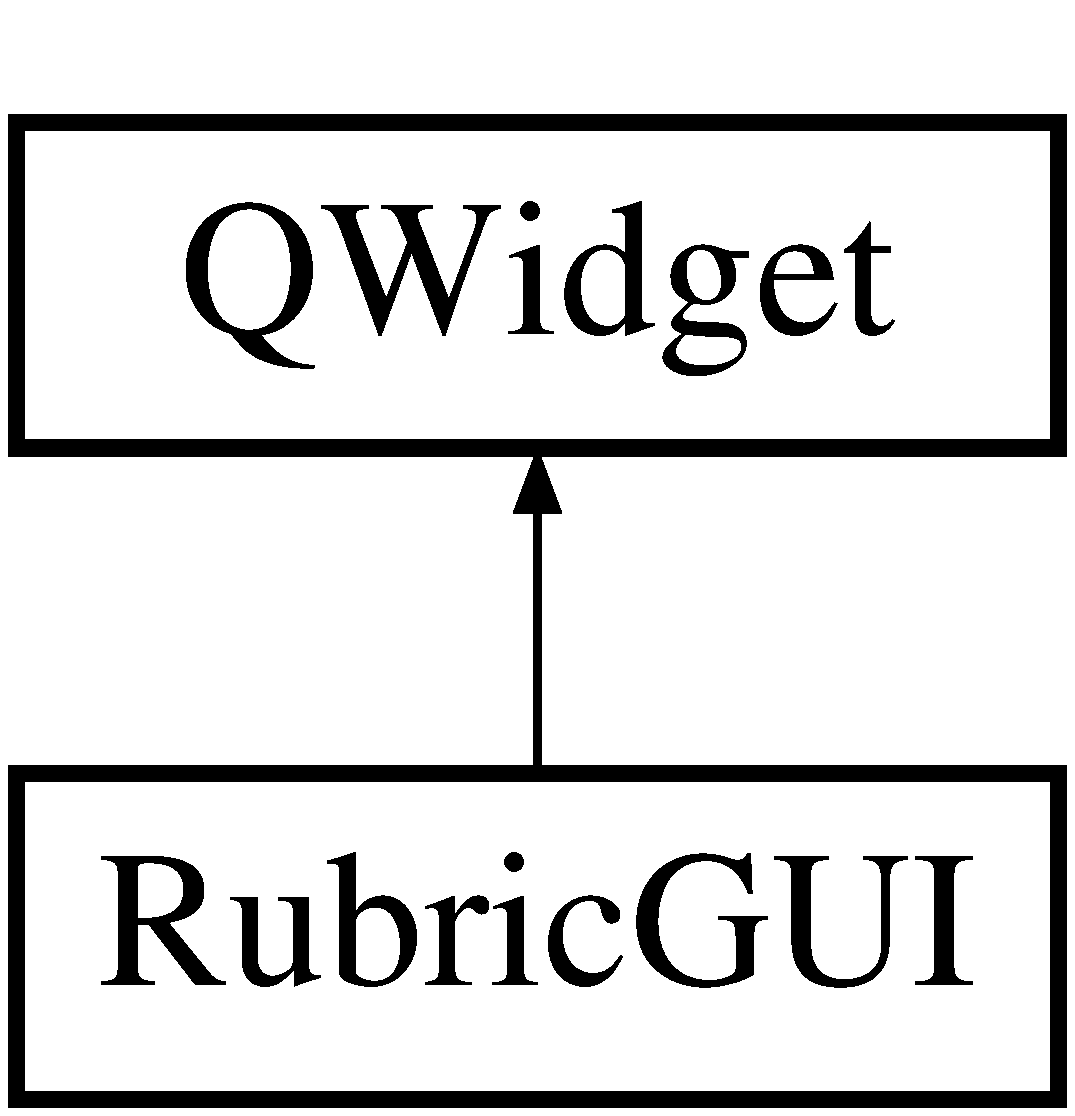
\includegraphics[height=2.000000cm]{class_rubric_g_u_i}
\end{center}
\end{figure}
\subsection*{Public Member Functions}
\begin{DoxyCompactItemize}
\item 
\hyperlink{class_rubric_g_u_i_a2cf12ba52cb750196813237dfd274116}{Rubric\+G\+UI} (Q\+Widget $\ast$parent=0, Grader $\ast$grad=nullptr)
\begin{DoxyCompactList}\small\item\em Rubric G\+UI header file. \end{DoxyCompactList}\item 
\hyperlink{class_rubric_g_u_i_a27ab6b386b6a42b7e2485ef75f4016e9}{$\sim$\+Rubric\+G\+UI} ()
\item 
void \hyperlink{class_rubric_g_u_i_a94675fa3481bd37ae6e3ed57967cb6e1}{display\+\_\+years} ()
\item 
\mbox{\Hypertarget{class_rubric_g_u_i_ab6b61d869f748fecaa2321fcc326d92f}\label{class_rubric_g_u_i_ab6b61d869f748fecaa2321fcc326d92f}} 
void {\bfseries display\+\_\+colors} ()
\end{DoxyCompactItemize}


\subsection{Constructor \& Destructor Documentation}
\mbox{\Hypertarget{class_rubric_g_u_i_a2cf12ba52cb750196813237dfd274116}\label{class_rubric_g_u_i_a2cf12ba52cb750196813237dfd274116}} 
\index{Rubric\+G\+UI@{Rubric\+G\+UI}!Rubric\+G\+UI@{Rubric\+G\+UI}}
\index{Rubric\+G\+UI@{Rubric\+G\+UI}!Rubric\+G\+UI@{Rubric\+G\+UI}}
\subsubsection{\texorpdfstring{Rubric\+G\+U\+I()}{RubricGUI()}}
{\footnotesize\ttfamily Rubric\+G\+U\+I\+::\+Rubric\+G\+UI (\begin{DoxyParamCaption}\item[{Q\+Widget $\ast$}]{parent = {\ttfamily 0},  }\item[{Grader $\ast$}]{a\+Grader = {\ttfamily nullptr} }\end{DoxyParamCaption})\hspace{0.3cm}{\ttfamily [explicit]}}



Rubric G\+UI header file. 

this class provides the set up and functionality for the rubric gui \begin{DoxyAuthor}{Author}
Allie Mullan 
\end{DoxyAuthor}
\begin{DoxyVersion}{Version}
2 constructor for the \hyperlink{class_rubric_g_u_i}{Rubric\+G\+UI}. Initializes the grader. Then calls methods to show the years and the colors in the proper gui dropdowns. 
\end{DoxyVersion}
\mbox{\Hypertarget{class_rubric_g_u_i_a27ab6b386b6a42b7e2485ef75f4016e9}\label{class_rubric_g_u_i_a27ab6b386b6a42b7e2485ef75f4016e9}} 
\index{Rubric\+G\+UI@{Rubric\+G\+UI}!````~Rubric\+G\+UI@{$\sim$\+Rubric\+G\+UI}}
\index{````~Rubric\+G\+UI@{$\sim$\+Rubric\+G\+UI}!Rubric\+G\+UI@{Rubric\+G\+UI}}
\subsubsection{\texorpdfstring{$\sim$\+Rubric\+G\+U\+I()}{~RubricGUI()}}
{\footnotesize\ttfamily Rubric\+G\+U\+I\+::$\sim$\+Rubric\+G\+UI (\begin{DoxyParamCaption}{ }\end{DoxyParamCaption})}

decostructor for the rubric gui. 

\subsection{Member Function Documentation}
\mbox{\Hypertarget{class_rubric_g_u_i_a94675fa3481bd37ae6e3ed57967cb6e1}\label{class_rubric_g_u_i_a94675fa3481bd37ae6e3ed57967cb6e1}} 
\index{Rubric\+G\+UI@{Rubric\+G\+UI}!display\+\_\+years@{display\+\_\+years}}
\index{display\+\_\+years@{display\+\_\+years}!Rubric\+G\+UI@{Rubric\+G\+UI}}
\subsubsection{\texorpdfstring{display\+\_\+years()}{display\_years()}}
{\footnotesize\ttfamily void Rubric\+G\+U\+I\+::display\+\_\+years (\begin{DoxyParamCaption}{ }\end{DoxyParamCaption})}

displays the years on the dropdown in the gui. 

The documentation for this class was generated from the following files\+:\begin{DoxyCompactItemize}
\item 
Rubric\+G\+U\+I/rubricgui.\+h\item 
Rubric\+G\+U\+I/rubricgui.\+cpp\end{DoxyCompactItemize}

%--- End generated contents ---

% Index
\backmatter
\newpage
\phantomsection
\clearemptydoublepage
\addcontentsline{toc}{chapter}{Index}
\printindex

\end{document}
